\documentclass{beamer}

\usetheme{focus} % Use the Focus theme supplied with the template
% Add option [numbering=none] to disable the footer progress bar
% Add option [numbering=fullbar] to show the footer progress bar as always full with a slide count

% Uncomment to enable the ice-blue theme
%\definecolor{main}{RGB}{92, 138, 168}
%\definecolor{background}{RGB}{240, 247, 255}

%------------------------------------------------

\usepackage{booktabs} % Required for better table rules
\usepackage[utf8]{inputenc}
\usepackage{tikz}
\usepackage{forest}
\usepackage{hhline}
\usepackage{multirow}

\usepackage{makecell}
\usepackage{subcaption}
\usepackage{caption}
\captionsetup{labelformat=empty,labelsep=none}
\usepackage{picture}
\usepackage[11pt]{moresize}
\usetikzlibrary{arrows.meta, shapes.geometric, calc, shadows}
\colorlet{linecol}{black!75}

%----------------------------------------------------------------------------------------
%	 TITLE SLIDE
%----------------------------------------------------------------------------------------

\title{Analysis of EEG-based Depression Biomarkers}

\subtitle{Using Machine Learning}

\author{Miroslav Kovář}

\titlegraphic{
\includegraphics[scale=1.25]{Images/lev.pdf}} % Optional title page image, comment this line to remove it

\institute{FJFI}

\date{\today}

%------------------------------------------------

\begin{document}
%------------------------------------------------

\begin{frame}
	\maketitle % Automatically created using the information in the commands above
\end{frame}

%----------------------------------------------------------------------------------------
%	 SECTION 1
%----------------------------------------------------------------------------------------

\section{Problem Statement and Approach} 
%------------------------------------------------
\begin{frame}{Depression Treatment is Expensive}
	\begin{columns}
		\column{0.5\textwidth}
        \begin{itemize}
          \item MDD
            \begin{itemize}
                % 800 000 suicides / year 
              \item<2-> 300 million suffering worldwide \cite{olbrich2013eeg, whodepression}
              \item<3-> diagnosis requires time of trained professionals \cite{whodepression}
            \end{itemize}
          \item EEG 
            \begin{itemize}
              \item<4-> accessible diagnosis-aid tool \cite{schultz2012}?
              \item<5-> also effective at prognosis? {\scriptsize studied very little!} 
            \end{itemize}
        \end{itemize}
        \vfill
        \visible<5->{Research into effective analysis techniques is ongoing\ldots}
		\column{0.5\textwidth}
            \begin{figure}
                \includegraphics<1->[width=0.9\linewidth]{./Images/electrodes.png}
                \caption{\scriptsize \cite{10-20-system}}
                % \\
                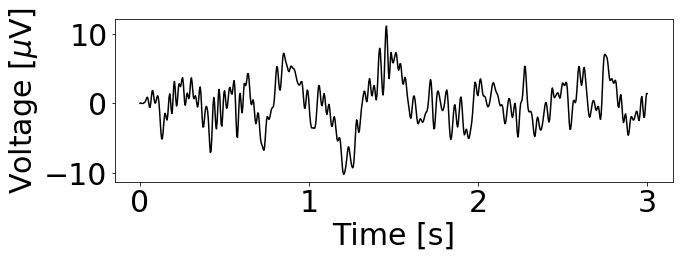
\includegraphics[width=\linewidth]{./Images/signal.png}
            \end{figure}
	\end{columns}
\end{frame}

%------------------------------------------------

\begin{frame}{Our Goals}
  \usetikzlibrary{arrows,positioning,decorations.pathreplacing}

\begin{tikzpicture}[
    every node/.style = {align=center},
          Line/.style = {-angle 90, shorten >=2pt},
    Brace/.style args = {#1}{semithick, decorate, decoration={brace,#1,raise=8pt,
                             pre=moveto,pre length=0pt,post=moveto,post length=0pt,amplitude=15pt}},
            ys/.style = {yshift=#1}
                    ]
\linespread{0.8}                    
\coordinate (a) at (0,0);
\coordinate[right=22mm of a]    (b);
\coordinate[right=18mm of b]    (c);
\coordinate[right= 5mm of c]    (d);
\coordinate[right=25mm of d]    (e);
\coordinate[right= 5mm of e]    (f);
\coordinate[right=10mm of f]    (g);

 \draw[Line]  (a)  --  (f) --  (g) node[below left] {weeks};
\foreach \x in {0,...,7} \draw (\x,0.1) -- (\x,-0.1) node[below] {\x};
\draw[Brace] (a) -- node[above=22pt] {Treatment}(e);
% \draw[Brace] (c) -- node[above=3pt] {Infectious period} (f);
% \draw[Brace=mirror] (d) -- node[below=3pt] {Symptomatic\\period} (e);
% \draw[Line] ([ys=11mm] a) node[above] {Time of\\infection} -- (a);
\draw[Line, shorten >=17pt] ([ys=-11mm]  c) node[below] {EEG recorded\\DS measured\\Prognosis} -- (c);
% \draw[Line] ([ys=7mm]  f) -- (f);
\draw[Line, shorten >=17pt] ([ys=-11mm] a) node[below] {Drugs administred\\EEG recorded\\DS measured\\Diagnosis} -- (a);\draw[Line, shorten >=17pt] ([ys=-11mm]  e) node[below]{Evaluation} -- (e);

\coordinate (a) at (0,-31mm);
\coordinate[right=22mm of a]    (b);
\coordinate[right=18mm of b]    (c);
\coordinate[right= 5mm of c]    (d);
\coordinate[right=25mm of d]    (e);
\coordinate[right= 5mm of e]    (f);
\coordinate[right=10mm of f]    (g);

 \draw[Line]  (a)  --  (f) --  (g) node[below left] {weeks};
\foreach \x in {0,...,7} \draw (\x,-32mm) -- (\x,-30mm) node[below=2mm] {\x};
% \draw[Brace] (a) -- node[above=22pt] {Treatment}(e);
% \draw[Brace] (c) -- node[above=3pt] {Infectious period} (f);
% \draw[Brace=mirror] (d) -- node[below=3pt] {Symptomatic\\period} (e);
% \draw[Line] ([ys=11mm] a) node[above] {Time of\\infection} -- (a);
\draw[Line, shorten >=17pt] ([ys=-11mm]  c) node[below] {EEG recorded\\DS measured\\\textcolor{red}{Evaluation}} -- (c);
% \draw[Line] ([ys=7mm]  f) -- (f);
\draw[Line, shorten >=17pt] ([ys=-11mm] a) node[below] {Drugs administred\\EEG recorded\\DS measured\\Diagnosis\\\textcolor{red}{Prognosis}} -- (a);
% \draw[Line, shorten >=17pt] ([ys=-11mm]  e) node[below]{Evaluation} -- (e);
\end{tikzpicture}
\end{frame}

%------------------------------------------------

\begin{frame}{Our Dataset}
	\begin{columns}
		\column{0.5\textwidth}
        \visible<1->{Relatively large:}
        \begin{itemize}
            \item<2-> 133 patients
            \item<3-> EEG recordings
              \begin{itemize}
                \item 19 channels
                \item 250 Hz or 1000 Hz
                \item Various duration
              \end{itemize}
              % \begin{itemize}
              %   \item 0 weeks
              %     \begin{itemize}
              %       \item Start of the treatment
              %       \item Drug administred
              %       \item Depression score measured
              %     \end{itemize}
              %   \item 4 weeks
              %     \begin{itemize}
              %       \item Depression score measured
              %     \end{itemize}
              % \end{itemize}
              \item<4-> Metadata
                  \begin{itemize}
                      \item Depression scores
                          \begin{itemize}
                              \item Week 0
                              \item Week 4
                          \end{itemize}
                       \item Age, gender, drugs
                  \end{itemize}
        \end{itemize}
        \vfill
        \visible<5->{Obtained from Czech National Institute of Mental Health}
		\column{0.5\textwidth}
			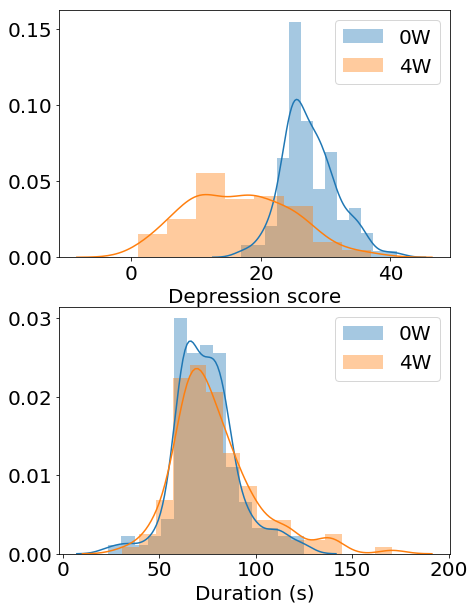
\includegraphics[width=\linewidth]{./Images/depscores_2.png}
	\end{columns}

\end{frame}

%------------------------------------------------

\begin{frame}[t]{Our Approach}

\pgfkeys{/forest,
  my rounded corners/.append style={rounded corners=2pt},
}
\centering
\scriptsize
\begin{forest}
for tree={
      % font=\sffamily,
      line width=1pt,
      draw=linecol,
      drop shadow,
      fit=rectangle,
      edge={thick, >={Triangle[]}, ->},
      where level=0{%
        l sep+=5pt,
        s sep=30mm,
        % calign=child,
        % calign child=1,
        % inner color=PaleGreen1!80,
        % outer color=PaleGreen1,
        % fill=green,
        top color=white, bottom color=blue!20,
        align=center,
        my rounded corners,
        for descendants={%
          calign=first,
        },
      }{%
        where level=1{%
          % inner color=green!80, outer color=green,
          top color=white, bottom color=blue!20,
          my rounded corners,
          align=center,
          parent anchor=west,
          tier=three ways,
          for descendants={%
            child anchor=west,
            parent anchor=west,
            align=left,
            anchor=west,
            % inner color=pink!80, outer color=pink,
            top color=white, bottom color=pink!20,
            edge path={%
              \noexpand\path[\forestoption{edge}]
              % (!to tier=three ways.parent anchor)|-(.child anchor)\forestoption{edge label};
              ($(!to tier=three ways.parent anchor)+(0.5\pgflinewidth,0)$)|-(.child anchor)\forestoption{edge label};
            },
          },
        }{}%
      },
  }
  [EEG Signals with Metadata, 
    [Nonlinear Analysis]
    [Deep Learning]
]
\end{forest}
\end{frame}

\begin{frame}[t]{Our Approach}
\pgfkeys{/forest,
  my rounded corners/.append style={rounded corners=2pt},
}
\centering
\scriptsize
\begin{forest}
for tree={
      % font=\sffamily,
      line width=1pt,
      draw=linecol,
      drop shadow,
      fit=rectangle,
      edge={thick, >={Triangle[]}, ->},
      where level=0{%
        l sep+=5pt,
        % calign=child,
        % calign child=1,
        % inner color=PaleGreen1!80,
        % outer color=PaleGreen1,
        % fill=green,
        top color=white, bottom color=blue!20,
        align=center,
        my rounded corners,
        for descendants={%
          calign=first,
        },
      }{%
        where level=1{%
          % inner color=green!80, outer color=green,
          top color=white, bottom color=blue!20,
          my rounded corners,
          align=center,
          parent anchor=west,
          tier=three ways,
          for descendants={%
            child anchor=west,
            parent anchor=west,
            align=left,
            anchor=west,
            % inner color=pink!80, outer color=pink,
            top color=white, bottom color=red!20,
            edge path={%
              \noexpand\path[\forestoption{edge}]
              % (!to tier=three ways.parent anchor)|-(.child anchor)\forestoption{edge label};
              ($(!to tier=three ways.parent anchor)+(0.5\pgflinewidth,0)$)|-(.child anchor)\forestoption{edge label};
            },
          },
        }{}%
      },
  }
  [EEG Signals with Metadata, 
    [Nonlinear Analysis
      [Preprocessing\\\scriptsize{labelling, curation}
          [State Space Reconstruction\\\scriptsize{embedding dimension, time lag,...}
            [Computing Measures\\\scriptsize{LLE, CD, DFA, HE, HD, SE}
              [Classification\\\scriptsize{LR, SVM}]
            ]
          ]
        ]
    ]
    [Deep Learning, 
      [Preprocessing\\\scriptsize{filtering}
          [Input Representation\\\scriptsize{RP, CS, raw data}
            [Architecture Design\\\scriptsize{CSP, FBCSP}
              [Classification\\\scriptsize{CNN}]
            ]
          ]
        ]
    ]
]
\end{forest}
\end{frame}

%----------------------------------------------------------------------------------------
%	 SECTION 2
%----------------------------------------------------------------------------------------

\section{Nonlinear Analysis Approach}

%------------------------------------------------

\begin{frame}{Nonlinear Measures}
  \begin{description}
  \item[LLE] Largest Lyapunov exponent
  \item[SE] Sample entropy         \makebox(0,0){\put(2.9cm,2.2\normalbaselineskip){%
                                   $\left.\rule{0pt}{1.1\normalbaselineskip}\right\}$ ``stability''}}
  \item[CD] Correlation dimension 
  \item[HD] Higuchi fractal dimension  \makebox(0,0){\put(1.2cm,2.2\normalbaselineskip){%
                                        $\left.\rule{0pt}{1.1\normalbaselineskip}\right\}$ ``complexity''}}
  \item[DFA] Detrended fluctuation analysis
  \item[HE] Hurst exponent              \makebox(0,0){\put(3cm,2.2\normalbaselineskip){%
                                        $\left.\rule{0pt}{1.1\normalbaselineskip}\right\}$ LRTC}}

  \end{description}
\end{frame}

%------------------------------------------------

\begin{frame}[t]{Embedding Parameter Estimation}
  \centering{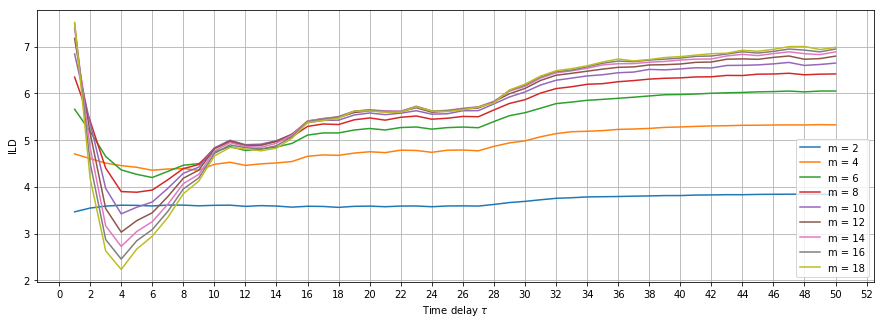
\includegraphics[width=\linewidth]{./Images/75b3.png}}
  \begin{columns}
    \column{0.5\textwidth}
    \textbf{Parameters}
      \begin{itemize}
        \item Embedding dimension
        \item Time delay
        \item Scaling regions
        \item \ldots
      \end{itemize}

    \column{0.5\textwidth}
    \textbf{Methods}
      \begin{itemize}
        \item Literature review
        \item Estimation algorithms (FNN, AFN, ADFD, ILD, \ldots)
        \item Statistical tests
      \end{itemize}
  \end{columns}
  \vfill
  \centering{\scriptsize{-> automated procedure}}
\end{frame}

%------------------------------------------------

\begin{frame}{Results}

\begin{table}[tbp]
% \ssmall
\fontsize{7pt}{10pt}
\selectfont
  \parbox{0.495\linewidth}{
\centering
\begin{tabular}{|c|c|c|c|}
\hline
\textbf{Measure} & \textbf{Classifier} & \multicolumn{2}{c}{\textbf{Accuracy}} \vline \\ \hline
& & \textbf{Mean} & \textbf{Std} \\ \hline
LLE, CD & SVM (lin.) & \textbf{0.74} & 0.04 \\ \hline 
LLE, SE & SVM (lin.) & 0.75 & 0.10 \\ \hline 
LLE, HE & SVM (lin.) & 0.73 & 0.06 \\ \hline 
LLE, SE, DFA & SVM (lin.) & 0.73 & 0.09 \\ \hline 
CD, HD & LR & 0.73 & 0.10 \\ \hhline{=|=|=|=}
LLE & SVM (lin.) & \textbf{0.72} & 0.04 \\ \hline
CD & SVM (lin.) & 0.71 & 0.05 \\ \hline 
SE & LR & 0.68 & 0.12 \\ \hline
HD & SVM (rbf) & 0.67 & 0.11 \\ \hline
DFA & LR & 0.67 & 0.16 \\ \hline
HE & LR & 0.67 & 0.17 \\ \hline
\end{tabular}
\subcaption{Depression}
}
\hfill
  \parbox{0.495\linewidth}{
\centering
\begin{tabular}{|c|c|c|c|}
\hline
\textbf{Measure} & \textbf{Classifier} & \multicolumn{2}{c}{\textbf{Accuracy}} \vline \\ \hline
& & \textbf{Mean} & \textbf{Std} \\ \hline
LLE, CD & SVM (lin.) & \textbf{0.75} & 0.11 \\ \hline 
LLE, SE & SVM (lin.) & 0.75 & 0.10 \\ \hhline{=|=|=|=}
LLE & LR & \textbf{0.71}  & 0.08 \\ \hline 
CD & LR & 0.67 & 0.09 \\ \hline
HD & LR & 0.66 & 0.05 \\ \hline
SE & LR & 0.66 & 0.09 \\ \hline
DFA & SVM (lin.) & 0.64 & 0.15 \\ \hline
HE & SVM (rbf) & 0.63 & 0.09 \\ \hline
\end{tabular}
\subcaption{Remission}
}
\end{table}
\end{frame}

%----------------------------------------------------------------------------------------
%	 SECTION 3
%----------------------------------------------------------------------------------------

\section{Deep Learning Approach}

%------------------------------------------------

\begin{frame}{Input Representation}
\begin{figure}
\centering
\begin{subfigure}{.5\textwidth}
  \centering
  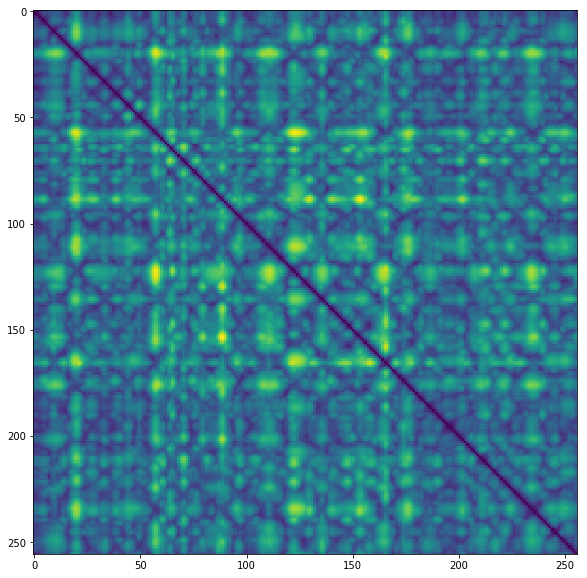
\includegraphics[width=.9\linewidth]{./Images/chebyshev.png}
  \caption{Recurrence plot}
  % \label{fig:sub1}
\end{subfigure}%
\begin{subfigure}{.5\textwidth}
  \centering
  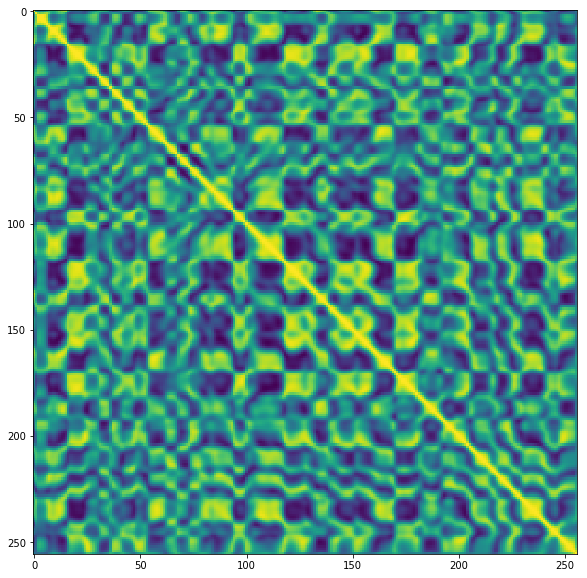
\includegraphics[width=.9\linewidth]{./Images/cs.png}
  \caption{Cosine similarity}
  % \label{fig:sub2}
\end{subfigure}
\end{figure}
\centering{\textbf{(c)} Raw}
\end{frame}

%------------------------------------------------

\begin{frame}{Architecture Design - Shallow}
  \centering
  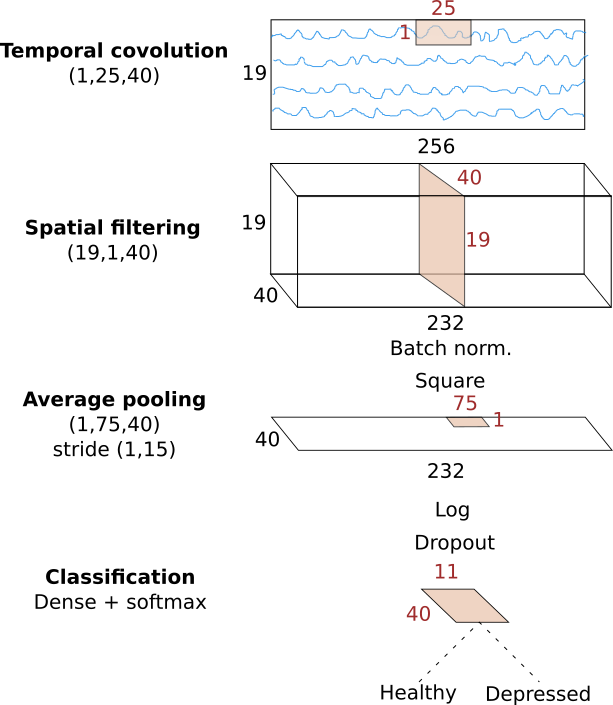
\includegraphics[width=0.6\linewidth]{./Images/shal.png}
\end{frame}

%------------------------------------------------

\begin{frame}{Architecture Design - Deep}
  \centering
  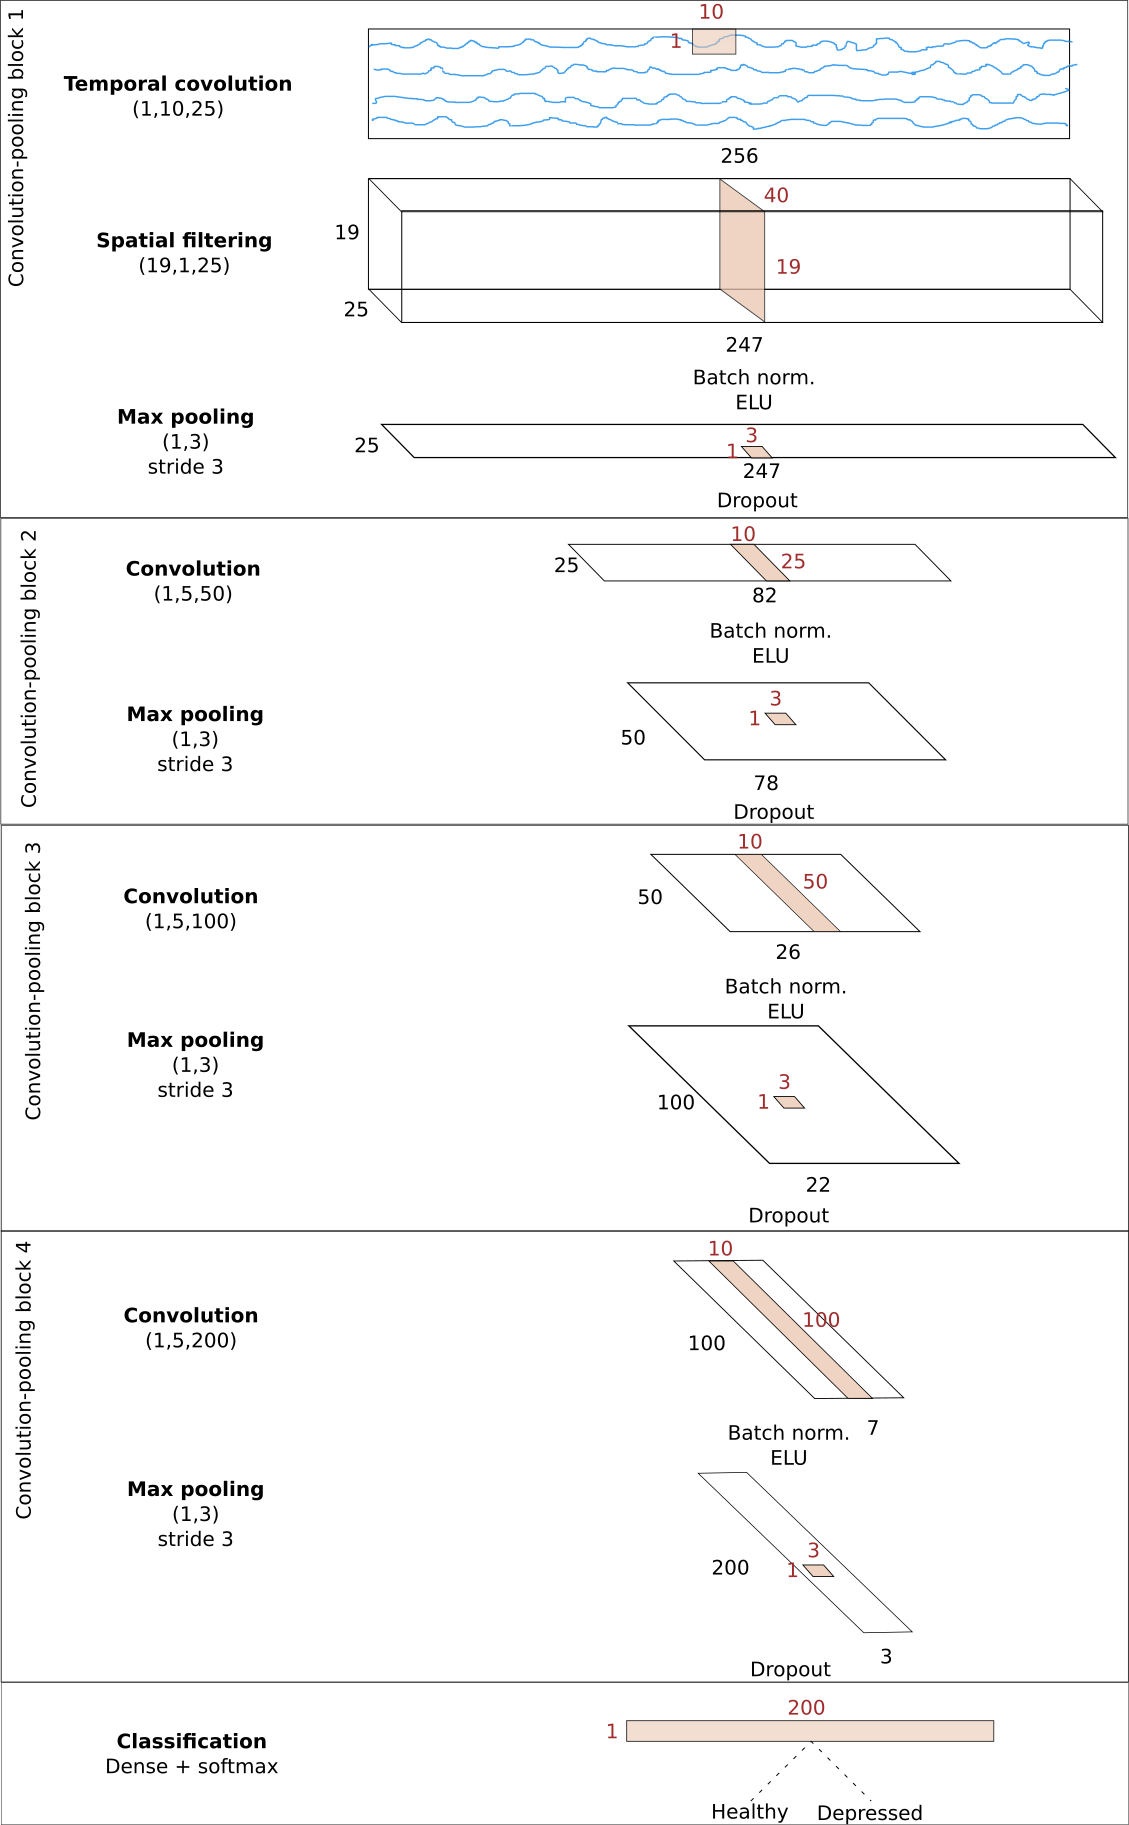
\includegraphics[width=0.4\linewidth]{./Images/deep.png}
\end{frame}

%------------------------------------------------

\begin{frame}{Results}
\begin{table}[tbp]
\centering
\scriptsize
  \parbox{0.495\linewidth}{
\centering
\begin{tabular}{|c|c|c|c|c|}
\hline
\textbf{Lab.} & \textbf{Freq.} & \textbf{Arch.} & \multicolumn{2}{c}{\textbf{Accuracy}} \vline \\ \hline
& & & \textbf{Mean} & \textbf{Std} \\ \hline
\multirow{4}{*}{DEP} & $0-f_{\text{fin}}$ & SHAL &  $0.85$ & $0.13$    \\ \cline{2-5}
                     & $4-f_{\text{fin}}$ & SHAL &     $0.84$ & $0.11$    \\ \cline{2-5} 
                     & $0-f_{\text{fin}}$ & DEEP &     $\mathbf{0.86}$ & $0.01$    \\ \cline{2-5} 
                     & $4-f_{\text{fin}}$ & DEEP &     $0.85$ & $0.02$    \\ \hline
\multirow{4}{*}{REM} & $0-f_{\text{fin}}$ & SHAL &  $\mathbf{0.94}$ & $0.02$    \\ \cline{2-5} 
                     & $4-f_{\text{fin}}$ & SHAL &     $0.94$ & $0.03$    \\ \cline{2-5} 
                     & $0-f_{\text{fin}}$ & DEEP &     $0.88$ & $0.01$    \\ \cline{2-5} 
                     & $4-f_{\text{fin}}$ & DEEP &     $0.86$ & $0.02$    \\ \hline
\end{tabular}
\subcaption{Raw data}
% \label{tab:depcl}
}
\hfill
  \parbox{0.495\linewidth}{
\centering
\begin{tabular}{|c|c|c|c|c|}
\hline
\textbf{Lab.} & \textbf{Freq.} & \textbf{Arch.} & \multicolumn{2}{c}{\textbf{Accuracy}} \vline \\ \hline
& & & \textbf{Mean} & \textbf{Std} \\ \hline
\multirow{4}{*}{DEP} & $0-f_{\text{fin}}$ & RP &   $\mathbf{0.63}$ & $0.02$ \\ \cline{2-5}      
                     & $4-f_{\text{fin}}$ & RP &      $0.61$ & $0.01$   \\ \cline{2-5}             
                     & $0-f_{\text{fin}}$ & CS &      $0.59$ & $0.02$  \\ \cline{2-5}              
                     & $4-f_{\text{fin}}$ & CS &      $0.58$ & $0.01$ \\ \hline
\multirow{4}{*}{REM} & $0-f_{\text{fin}}$ & RP &   $0.61$ & $0.03$ \\ \cline{2-5}               
                     & $4-f_{\text{fin}}$ & RP &       $\mathbf{0.65}$ & $0.02$    \\ \cline{2-5}   
                     & $0-f_{\text{fin}}$ & CS &      $0.55$ & $0.02$ \\ \cline{2-5}               
                     & $4-f_{\text{fin}}$ & CS &      $0.63$ & $0.01$ \\ \hline               
\end{tabular}
\subcaption{Image-encoded data}
% \label{tab:depcl}
}
\end{table}
\end{frame}

%----------------------------------------------------------------------------------------
%	 SECTION 3
%----------------------------------------------------------------------------------------

\section{Conclusion}

%------------------------------------------------

\begin{frame}{Summary}
    \centering
    \begin{enumerate}
        \item NL measures are potentially effective methods for depression diagnosis and prognosis {\scriptsize(despite nonstationarity)}
        \item CD and LLE seem most discriminative {\scriptsize{(out of evaluated)}}
            % CD is especially surprising, since no scaling region was found!
        \item FBCSP-inspired CNN models seem more effective than common models
        {\scriptsize
        \item ILD seems most effective embedding parameters estimation algorithm {\scriptsize(out of evaluated)}
        \item RP and CS do not seem effective data encoding methods for EEG analysis
        }
    \end{enumerate}
    
\end{frame}

%------------------------------------------------

\begin{frame}[t]{Summary}
  \centering
  \begin{columns}[t]
    \column{0.5\linewidth}
    \centering{\textbf{Limitations}}
    \begin{itemize}
      \item Binary output
      \item Most patients in remission % i.e. the classes may have been artifically balanced, not enough non-remitting patients
    \end{itemize}
    \centering{\textbf{\footnotesize{NL approach}}}
        \begin{itemize}
          \item Nonstationarity {\scriptsize (windowing?)} 
          \item Spatially local % i.e. impossible to detect spatial features, difficult to predict temporal
          \item Temporally global
          \item Inconclusive surrogate tests
          \item ``Theoretically too ambitious''
        \end{itemize}
    \centering{\textbf{\footnotesize{DL approach}}}
        \begin{itemize}
          \item Short samples
          \item Simple models
        \end{itemize}

    \column{0.5\linewidth}
    \centering{\textbf{Future Work}}
    \scriptsize
    \begin{itemize}
      \item Implement application to aid treatment
      \item Generalization to other datasets {\scriptsize (sample bias) }
      \item Output depression severity measure
      \item Ensemble of models combining (neuroimaging) modalities
      \item Incorporate information about treatment details (drugs,\ldots)
    \end{itemize}
    \centering{\textbf{\scriptsize{NL approach}}}
        \begin{itemize}
          \item Compare with spatial embedding
          \item New (spatiotemporal) measures
        \end{itemize}
    \centering{\textbf{\scriptsize{DL approach}}}
        \begin{itemize}
          \item Model interpretation % {\scriptsize Do CNNs compute NL measures?}
          \item Compare with FBCSP
          \item Dimensionality reduction techniques
        \end{itemize}
  \end{columns}
\end{frame}

%------------------------------------------------

\begin{frame}[focus]
  \textbf{Questions}
\end{frame}

%----------------------------------------------------------------------------------------
%	 CLOSING/SUPPLEMENTARY SLIDES
%----------------------------------------------------------------------------------------

\appendix

\begin{frame}[allowframebreaks]{References}
	% \nocite{*} % Display all references regardless of if they were cited
	\bibliography{../refs.bib}
	\bibliographystyle{plain}
\end{frame}

%------------------------------------------------

\begin{frame}{Backup Slides}
\end{frame}

%----------------------------------------------------------------------------------------

\end{document}
